\documentclass{article}
\usepackage{iclr2027_conference,times}
\usepackage{amsmath,amssymb}
\usepackage{booktabs}
\usepackage{graphicx}
\usepackage{hyperref}
\usepackage{microtype}
\usepackage{url}
\usepackage{xcolor}
\newcommand{\ResultPreset}{full}
\newcommand{\MaxN}{128}
\newcommand{\SymbolicNOneUtility}{37.3}
\newcommand{\SymbolicMaxUtility}{15.9}
\newcommand{\SymbolicMaxLoophole}{100.0\%}
\newcommand{\SymbolicGap}{109.8}
\newcommand{\SimulatorMaxUtility}{15.9}
\newcommand{\SimulatorMaxLoophole}{100.0\%}
\newcommand{\CalibratedUtility}{84.6}
\newcommand{\AdversarialUtility}{84.6}
\newcommand{\LCBUtility}{84.6}
\newcommand{\BestRepairName}{calibrated\_boundary}
\newcommand{\BestRepairUtility}{84.6}
\newcommand{\BestRepairSuccess}{100.0\%}
\newcommand{\BestRepairLoophole}{0.0\%}
\newcommand{\StressMaxN}{512}
\newcommand{\StressSymbolicUtility}{15.9}
\newcommand{\StressSymbolicLoophole}{100.0\%}
\newcommand{\StressSymbolicSuccess}{0.0\%}
\newcommand{\StressSimulatorUtility}{15.9}
\newcommand{\StressAdversarialUtility}{84.6}
\newcommand{\StressLCBUtility}{84.6}
\newcommand{\StressRarePriorLoophole}{100.0\%}
\newcommand{\StressStrictSuccess}{100.0\%}
\newcommand{\StressProxyAdvantage}{69.0}
\newcommand{\StressGroundedAdvantage}{60.6}
\newcommand{\FrozenMaxN}{128}
\newcommand{\FrozenNOneUtility}{40.1}
\newcommand{\FrozenSymbolicUtility}{0.0}
\newcommand{\FrozenSymbolicSuccess}{0.0\%}
\newcommand{\FrozenSymbolicHole}{100.0\%}
\newcommand{\FrozenSimulatorUtility}{0.0}
\newcommand{\FrozenHazardGateUtility}{93.0}
\newcommand{\FrozenHazardGateSuccess}{100.0\%}
\newcommand{\FrozenLCBUtility}{93.0}
\newcommand{\FrozenLCBSuccess}{100.0\%}
\newcommand{\FrozenHazardProxyAdvantage}{22.1}
\newcommand{\FrozenSafeUtilityAdvantage}{93.0}


\hypersetup{
  colorlinks=true,
  linkcolor=black,
  citecolor=black,
  urlcolor=blue
}

\title{\vspace{-0.5em}Plans That Pass But Do Not Execute:\\
Boundary Audits for Language-to-Symbolic Planning}

% The ICLR submission style keeps this anonymous while \iclrfinalcopy is commented.
\author{Anonymous Authors}

%\iclrfinalcopy

\begin{document}
\maketitle

\begin{abstract}
Language/symbolic planner hybrids often generate several natural-language plan
candidates, compile each candidate into symbolic actions, and choose a plan that
passes a checker or scores well under a simulator proxy. This paper isolates a
failure mode at that boundary: a plan can satisfy the symbolic interface while
violating hidden execution semantics omitted from the abstraction. We construct
small deterministic language-to-action domains with a coarse checker, surrogate
simulator, and stricter hidden executor. A two-type finite-pool argument shows
that if boundary-loophole plans receive higher proxy scores but lower true
utility than grounded plans, increasing the candidate budget raises the
probability of selecting a loophole to $1-(1-p)^N$ and decreases expected true
utility. In the full local run, symbolic-proxy selection drops from
\SymbolicNOneUtility{} true utility at $N=1$ to \SymbolicMaxUtility{} at
$N=\MaxN{}$, with \SymbolicMaxLoophole{} selected-loophole occupancy and a
\SymbolicGap{} mean proxy-true gap. Simulator-proxy selection shows the same
collapse. Semantic uncertainty penalties and adversarial execution gates recover
grounded plans in this controlled setting. The claim is intentionally narrow:
this is a boundary-audit scaffold, not evidence about deployed robotics systems.
\end{abstract}

\section{Introduction}

Language models are increasingly used as planners, translators to symbolic
languages, tool-using agents, and proposal generators for robot or simulator
controllers. The usual safety hope is modular: a symbolic checker, simulator, or
verifier should catch invalid plans before execution. A language model proposes
candidates, the symbolic layer validates or ranks them, and the system executes
the apparently valid plan.

This paper studies a failure of that modular hope. The dangerous object is not a
plan that obviously violates the checker. It is a plan that crosses the
language-to-symbolic boundary in a way that is locally valid but semantically
incomplete: paperwork satisfies a delivered predicate without a physical
handoff, a service elevator gives symbolic reachability while contaminating a
sterile kit, or a signed form is treated like moving an archive box. These
loopholes can be rare in the generator but preferred by the proxy once they
appear in the candidate pool.

Our contributions are:
\begin{enumerate}
  \item a compact mechanism law for boundary-loophole amplification under
  proxy-ranked candidate-pool selection;
  \item a deterministic toy benchmark that separates language prior, symbolic
  checker, simulator proxy, and hidden execution utility; and
  \item diagnostics and simple repair gates that test whether selected plans
  depend on missing boundary semantics.
\end{enumerate}

The paper is deliberately small. It does not introduce a planner architecture or
claim external robotics validity. Its purpose is to provide an audit that can be
run before trusting a symbolic interface as an execution guarantee.

\section{Related Work}

LLM+P and related language-to-PDDL systems show how language models can call
classical planners rather than solve planning internally. ReAct, SayCan, Inner
Monologue, Code as Policies, Voyager, and Reflexion explore language agents,
affordances, tools, and feedback loops. Tree of Thoughts and self-consistency
are close inference-time search ancestors. Reward-model and verifier-hacking
work warns that optimizing an imperfect proxy can expose misspecification. Our
contribution is narrower than these lines: it isolates the selection pressure
created when language-generated plans cross a symbolic abstraction boundary
before execution.

The repository includes a related-work matrix, literature map, hostile
prior-work memo, and novelty decision. That audit led us away from claiming a
new agent method and toward a mechanism-level diagnostic for checker/executor
divergence.

\section{Mechanism}

Consider candidate plans sampled independently. Let a candidate be a boundary
loophole with probability $p>0$ and a grounded plan otherwise. Suppose every
loophole receives proxy score $s_L$ and every grounded plan receives $s_G$, with
$s_L>s_G$, but true utilities satisfy $u_L<u_G$. A top-proxy selector chooses a
loophole whenever at least one loophole appears:
\[
P(\text{loophole selected}) = 1-(1-p)^N.
\]
Thus expected true utility is
\[
\mathbb{E}[u_N] = \left(1-(1-p)^N\right)u_L + (1-p)^Nu_G,
\]
which decreases monotonically to $u_L$. The proposition is not deep probability;
its value is diagnostic. It says a checker can be locally correct relative to
its symbols while the selection procedure globally amplifies missing semantics.

\section{Controlled Domains}

Each domain has language-like candidate plans, a compiler to symbolic actions, a
coarse checker, a surrogate simulator score, and a hidden executor. The checker
tracks location, possession, unlock status, and a delivered predicate. The
executor additionally tracks physical transfer, carrier/packing, PPE, and
contamination.

Candidate modes include robust grounded plans, lean unsealed plans, invalid
plans, paperwork loopholes, service-elevator shortcuts, and simulator lures. The
symbolic checker accepts paperwork completion as delivery and treats shortcut
transitions as certified reachability. The executor scores those candidates
poorly because no physical handoff occurred or the item is contaminated.

\section{Selectors and Diagnostics}

We compare random valid selection, language-prior selection, symbolic-proxy
selection, simulator-proxy selection, calibrated boundary penalties, an
adversarial execution gate, and an uncertainty lower-confidence-bound selector.
The repair selectors are deliberately simple. They penalize features that expose
semantic uncertainty: goal completion without physical delivery, shortcut
transitions, missing packing, and declarations unsupported by state.

The audit reports selected true utility, execution success, selected loophole
occupancy, semantic-bad rate, proxy-true gap, checker pass rate, and pool-level
execution success. The strongest diagnostic is not generic regret; it is whether
the selected plan uses an abstraction-boundary loophole.

\section{Results}

Figure~\ref{fig:collapse} shows the central scaling curve. Symbolic-proxy and
simulator-proxy selection improve the proxy objective but select lower-utility
plans as $N$ grows. At $N=\MaxN{}$, symbolic-proxy selection reaches
\SymbolicMaxLoophole{} loophole occupancy and \SymbolicMaxUtility{} true
utility; simulator-proxy selection reaches \SimulatorMaxLoophole{} loophole
occupancy and \SimulatorMaxUtility{} true utility.

Figure~\ref{fig:loophole} shows the selected-plan mechanism directly: loophole
occupancy rises with $N$ for unrepaired proxy selectors. Figure~\ref{fig:gap}
shows that checker pass rate and execution success are distinct quantities.
Figure~\ref{fig:repair} summarizes the repair ladder at the largest $N$. The
best repair in the full run is \BestRepairName{}, with \BestRepairUtility{}
true utility, \BestRepairSuccess{} execution success, and \BestRepairLoophole{}
loophole occupancy.

\clearpage

\begin{figure}[t]
\centering
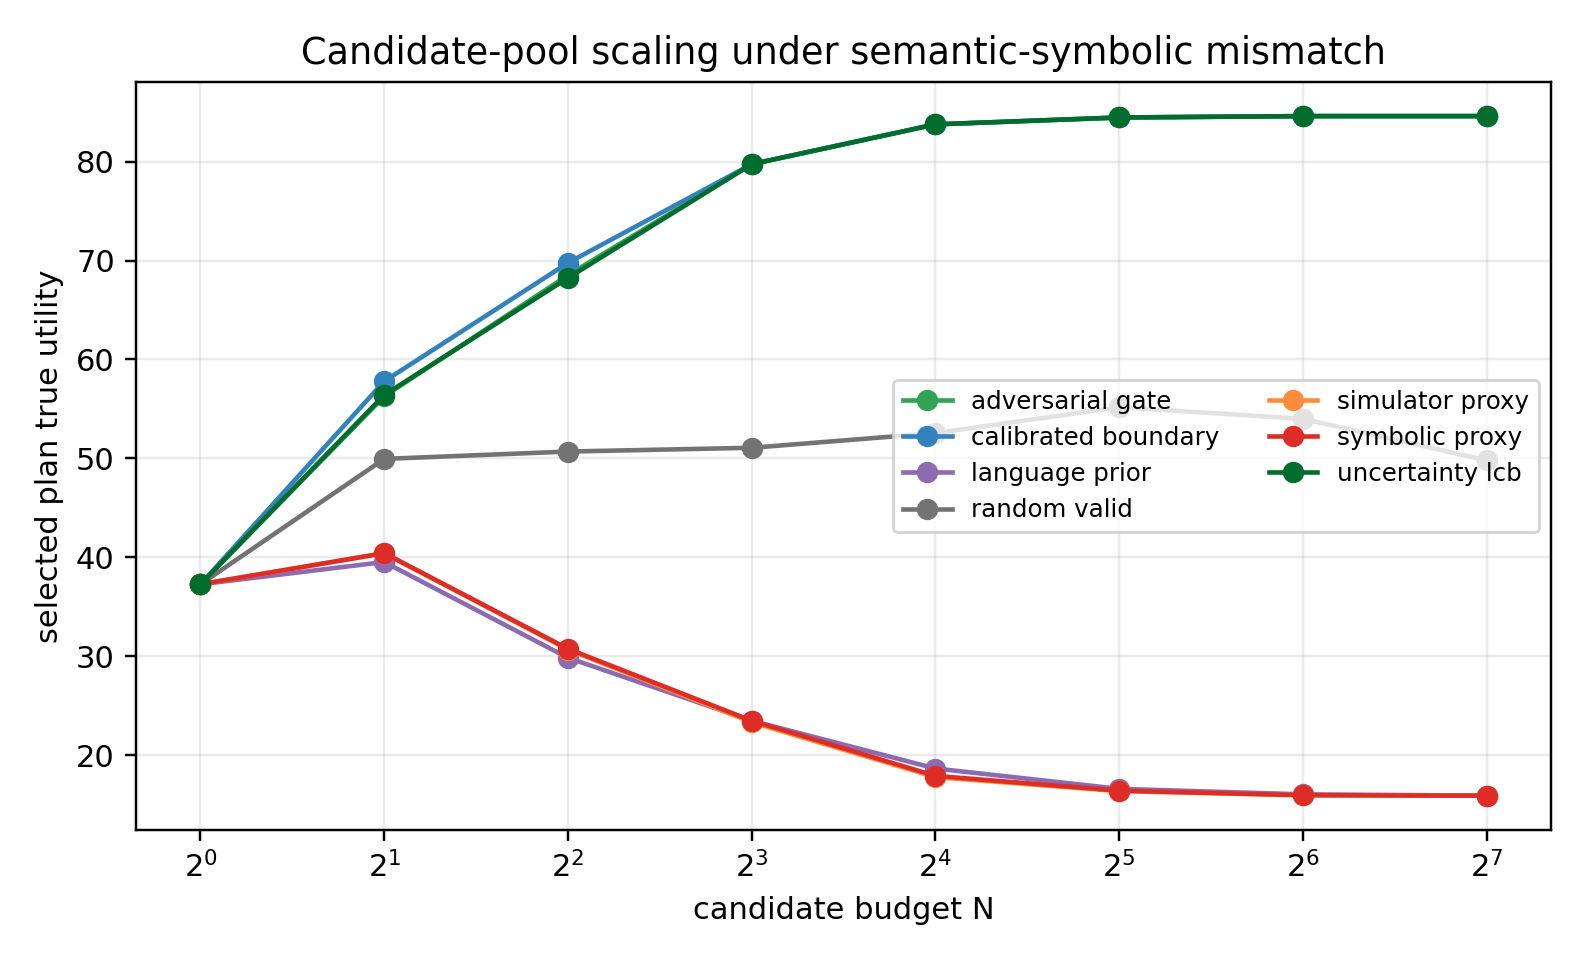
\includegraphics[width=\linewidth]{../figures/full/figure1_boundary_collapse.png}
\caption{True utility of the selected plan as candidate budget grows. Proxy
selectors collapse once rare boundary loopholes appear; repaired selectors
recover grounded execution in these toy domains.}
\label{fig:collapse}
\end{figure}

\begin{figure}[t]
\centering
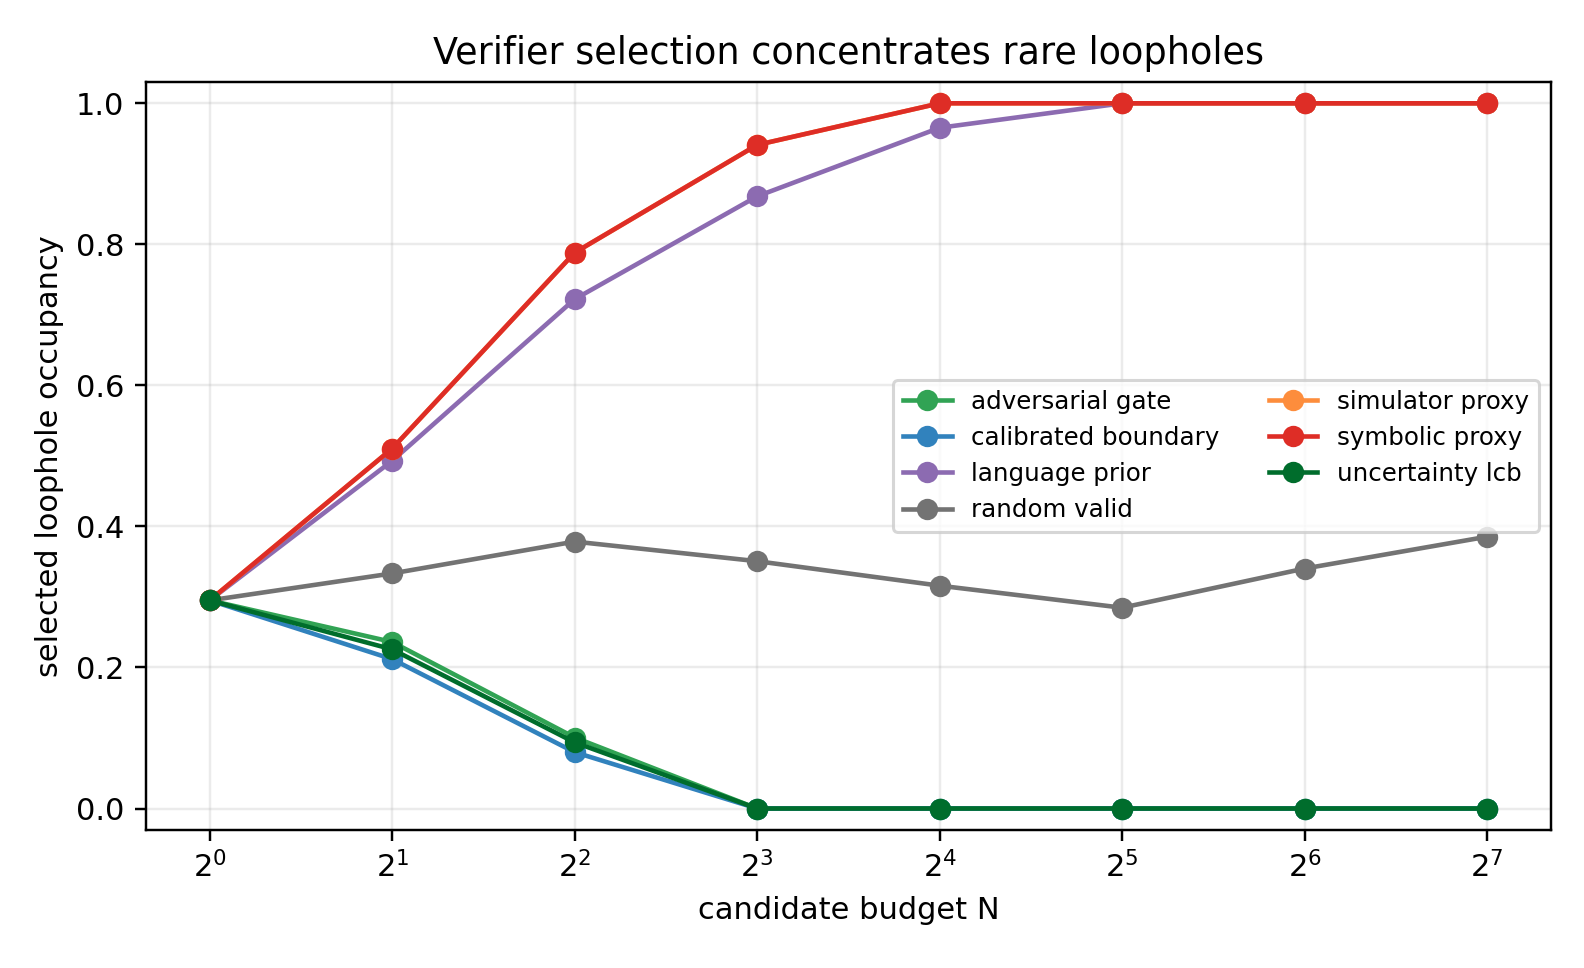
\includegraphics[width=\linewidth]{../figures/full/figure2_loophole_occupancy.png}
\caption{Selected loophole occupancy. The diagnostic asks whether the selected
plan exploits the abstraction boundary, not merely whether proxy regret grows.}
\label{fig:loophole}
\end{figure}

\begin{figure}[t]
\centering
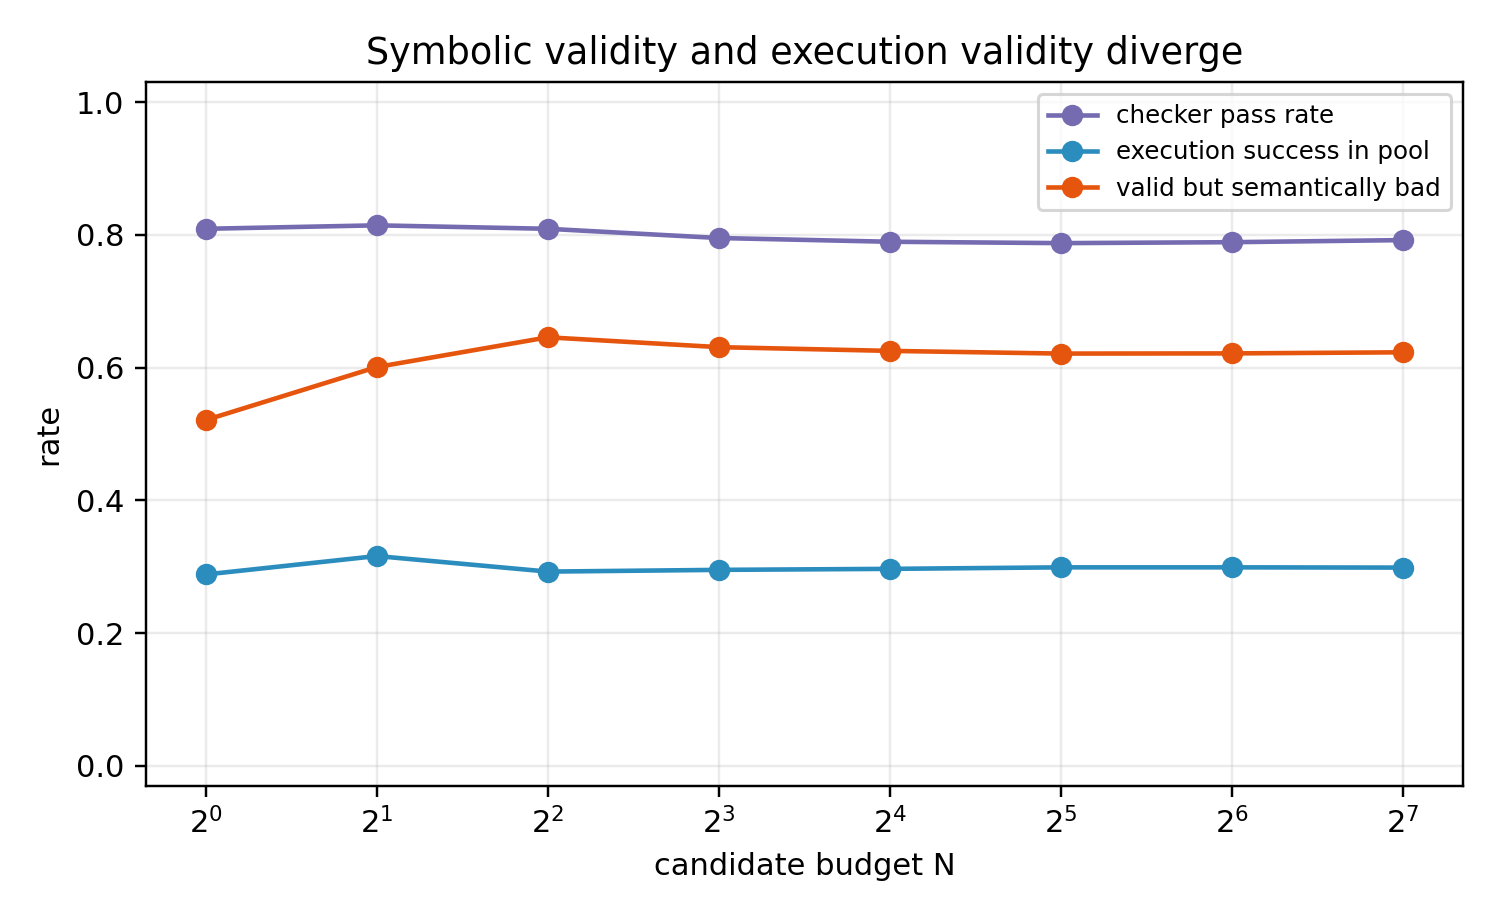
\includegraphics[width=\linewidth]{../figures/full/figure3_checker_executor_gap.png}
\caption{Pool-level checker/executor gap. Symbolic pass rate is not execution
success when the abstraction omits hidden task semantics.}
\label{fig:gap}
\end{figure}

\begin{figure}[t]
\centering
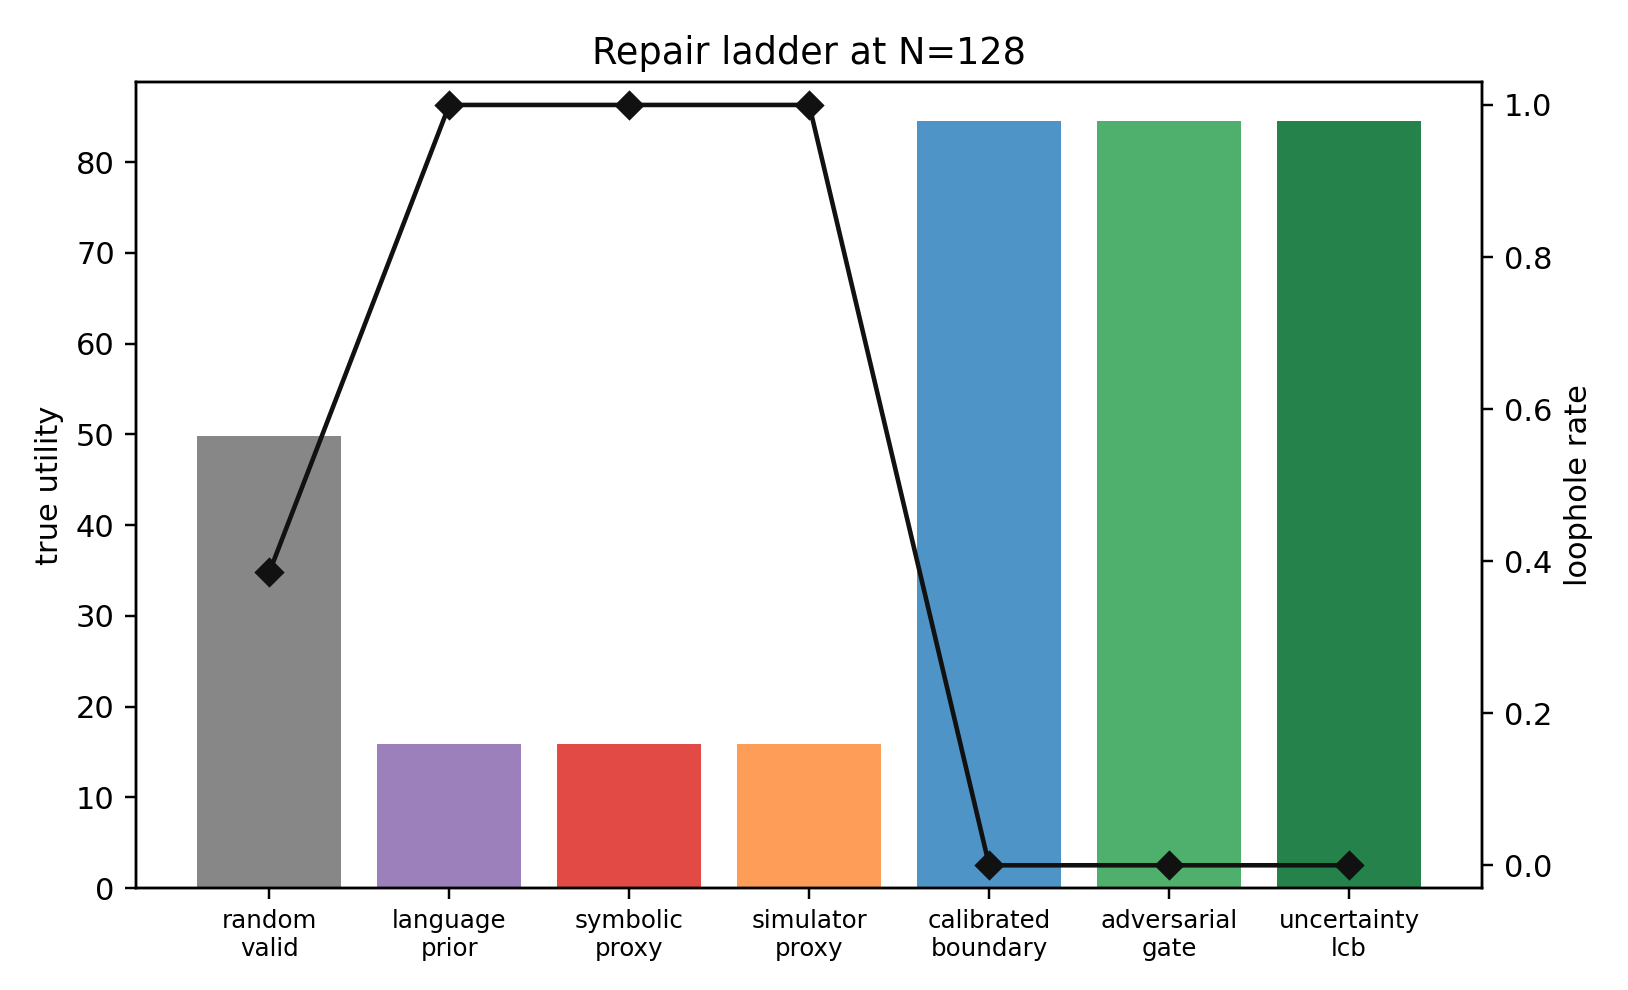
\includegraphics[width=\linewidth]{../figures/full/figure4_repair_ladder.png}
\caption{Repair ladder at the largest candidate budget. Semantic uncertainty
and adversarial gates reduce the controlled mismatch.}
\label{fig:repair}
\end{figure}

\clearpage

\section{Limitations}

The domains are synthetic and intentionally small. The language generator is a
stochastic template model, not a frontier LLM. The simulator is handcrafted to
expose a mechanism, not learned from large-scale data. The repair gates use
privileged feature knowledge and should be read as diagnostics, not
deployment-ready safety tools. The paper supports architecture-specific
mechanism claims, not broad claims about robot safety or all symbolic
verification.

\section{Reproducibility and Ethics}

All experiments are CPU-only, deterministic under fixed seeds, and require no
external APIs. The work is defensive: it identifies a way proxy validation can
overstate execution readiness. The main misuse risk is overgeneralizing the toy
result, which is why the repository includes claim audits and unsupported-claim
lists.

\section{Checklist}
\begin{itemize}
\item Anonymous submission: yes.
\item Code and data: included in the repository; generated outputs are under
\texttt{results/} and \texttt{figures/}.
\item Compute: CPU-only Python suite.
\item Limitations: stated above and in \texttt{docs/final\_audit.md}.
\item Claims: controlled synthetic mechanism only.
\end{itemize}

\begin{thebibliography}{9}
\bibitem[Liu et~al.(2023)]{llmp} Liu et al. LLM+P: Empowering Large Language Models with Optimal Planning Proficiency. arXiv, 2023.
\bibitem[Yao et~al.(2023a)]{react} Yao et al. ReAct: Synergizing Reasoning and Acting in Language Models. ICLR, 2023.
\bibitem[Ahn et~al.(2022)]{saycan} Ahn et al. Do As I Can, Not As I Say: Grounding Language in Robotic Affordances. CoRL, 2022.
\bibitem[Huang et~al.(2022)]{inner} Huang et al. Inner Monologue: Embodied Reasoning through Planning with Language Models. CoRL, 2022.
\bibitem[Yao et~al.(2023b)]{tot} Yao et al. Tree of Thoughts: Deliberate Problem Solving with Large Language Models. NeurIPS, 2023.
\bibitem[Wang et~al.(2023)]{selfconsistency} Wang et al. Self-Consistency Improves Chain of Thought Reasoning in Language Models. ICLR, 2023.
\bibitem[Liang et~al.(2023)]{codepolicies} Liang et al. Code as Policies: Language Model Programs for Embodied Control. ICRA, 2023.
\bibitem[Everitt et~al.(2021)]{rewardtamper} Everitt et al. Reward Tampering Problems and Solutions in Reinforcement Learning. Synthese, 2021.
\end{thebibliography}

\end{document}
